\documentclass[a4paper]{article}

\usepackage{amsmath}
\usepackage{amssymb}
\usepackage{hyperref}
\usepackage{graphicx}

\newcommand{\BITZ}{\mathop{\rm BIT0}}
\newcommand{\BITO}{\mathop{\rm BIT1}}
\newcommand{\SUC}{\mathop{\rm SUC}}
\newcommand{\linf}{\mathop{\rm linf}}
\newcommand{\issues}{{\bf Known issues:}\\}
\newcommand{\xx}[1]{\mathop{\text{\bf #1}}}

\parindent=0mm
\parskip=5pt

\title{SSReflect/HOL Light}

\author{Alexey Solovyev}

% Document
\begin{document}
% Title
\maketitle

% Content
\tableofcontents

\pagebreak
\section{Getting Started}

% References
\subsection{References}
\begin{itemize}
\item[1.] HOL Light home page\\ 
	\url{http://www.cl.cam.ac.uk/~jrh13/hol-light}
\item[2.] HOL Light reference manual\\
	\url{http://www.cl.cam.ac.uk/~jrh13/hol-light/reference.html}
\item[3.] HOL Light tutorial\\
	\url{http://www.cl.cam.ac.uk/~jrh13/hol-light/tutorial_220.pdf}
\item[4.] Mathematical Components project at MS Research--INRIA\\
	\url{http://www.msr-inria.inria.fr/Projects/math-components}
\item[5.] SSReflect tutorial\\
	\url{http://www.msr-inria.inria.fr/Projects/math-components/tutorial.pdf}
\item[6.] SSReflect reference manual\\
	\url{http://hal.inria.fr/inria-00258384}
\item[7.] The Flyspeck project\\
	\url{http://code.google.com/p/flyspeck/}
\end{itemize}

% Introduction
\subsection{Introduction}
SSReflect is a special language for formalizing mathematics in Coq proof assistant. It was developed by Georges Gonthier at Microsoft Research--INRIA Joint Center. In this document I present my implementation of SSReflect language for doing proofs in HOL Light proof assistant. My system (which I will call SSReflect/HOL Light, and the original language will be called SSReflect/Coq) is not a complete reimplementation of SSReflect in HOL Light. I implemented a subset of the language which I personally think is useful for writing proofs in HOL Light in a more efficient way than with a standard HOL Light proof script.

I assume that a reader is familiar with HOL Light proof assistant. Knowledge of SSReflect/Coq is helpful, but it is not required to understand and use my SSReflect/HOL Light system for creating HOL Light proofs.

% Installation
\subsection{Installation}
The requirements to run SSReflect/HOL Light are:
\begin{itemize}
\item A Java runtime of version 1.5 or higher.
\item A checkpointed version of HOL Light.
\item A script which can load a checkpointed version of HOL Light. This script must be on the system path.
\end{itemize}

The distribution of SSReflect/HOL Light can be downloaded at

\url{http://flyspeck.googlecode.com/files/HOL-SSReflect.zip}

The distribution includes a compiled version of the source code, the source code itself, and all supporting files.

The installation process is simple: extract the distribution archive into any directory. Then SSReflect/HOL Light can be started with the following command

\verb|java -jar jHOL-SSReflect.jar [name of a HOL Light loading script]|

By default, it is assumed that a HOL Light loading script has the name \verb|hol_light|. Any other name can be provided as the command argument. A version of HOL Light loaded by the script must contain \verb|"."| in the \verb|load_path| variable (alternatively, \verb|load_path| may contain the path to the directory where {\tt jHOL-SSReflect.jar} is located).

\issues
On my computer, SSReflect/HOL Light does not work with a checkpointed version of HOL Light created with Berkeley Checkpoint/Restart (BLCR). I use DMTCP checkpointing to run HOL Light with SSReflect/HOL Light. I didn't test any other checkpointing software.


% Implementation
\subsection{Implementation Notes}
SSReflect/HOL Light is implemented in Java and OCaml. The Java part includes a user interface, which can understand and print HOL Light terms, and a translator of SSReflect/HOL Light commands and tactics into OCaml. The OCaml part implements special HOL Light tactics.

The project is located at the {\tt jHOLLight} directory of the Flyspeck repository. The directory {\tt jHOLLight/caml} contains OCaml files of the project. This directory contains the following files related to the OCaml part of the system:
\begin{itemize}
\item {\tt raw\_printer.hl} -- a special HOL Light term converter which produces strings of symbols that can be parsed by the Java part of the system.
\item {\tt ssreflect.hl} -- special HOL Light tactics.
\item {\tt sections.hl} -- a simple section mechanism in HOL Light.
\end{itemize}

The main source code packages are:
\begin{itemize}
\item {\tt jHOLLight/src/edu/pitt/caml} -- classes which correspond to Caml types and objects.
\item {\tt jHOLLight/src/edu/pitt/core} -- classes which correspond to HOL Light terms and theorems.
\item {\tt jHOLLight/src/edu/pitt/core/parser} -- a parser of a special representation of HOL Light terms which is produced by {\tt raw\_printer.hl}.
\item {\tt jHOLLight/src/edu/pitt/core/printer} -- a printer of HOL Light terms.
\item {\tt jHOLLight/src/edu/pitt/gui} -- UI components for displaying terms and theorems.
\item {\tt jHOLLight/src/edu/pitt/ssreflect/gui} -- SSReflect/HOL Light user interface.
\item {\tt jHOLLight/src/edu/pitt/ssreflect/parser} -- SSReflect/HOL Light translator.
\end{itemize}


% Examples
\subsection{Examples}
I translated several basic SSReflect/Coq libraries into SSReflect/HOL Light. These libraries are {\tt ssrnat.vhl} and {\tt seq.vhl} ({\tt .vhl} is the extension which I chose for SSReflect/HOL Light script files) and they can be found in the {\tt caml} directory of the distribution of SSReflect/HOL Light.

I also experimented with some group theory in SSReflect/HOL Light and proved Sylow theorems. It can be found in the file {\tt group\_sylow.vhl} in the {\tt caml} directory. 

Several results about second order Taylor approximations of univariate and multivariate functions was proved with SSReflect/HOL Light. This theory is used in my HOL Light procedure for verification of non-linear inequalities. Theory files are contained in the Flyspeck repository at {\tt svn/trunk/formal\_lp/formal\_interval/theory} and they are called {\tt taylor\_interval.vhl} and {\tt multivariate\_taylor.vhl}.


% IDE
\section{IDE}

% Overview
\subsection{Overview}
\begin{figure}
\label{gui}
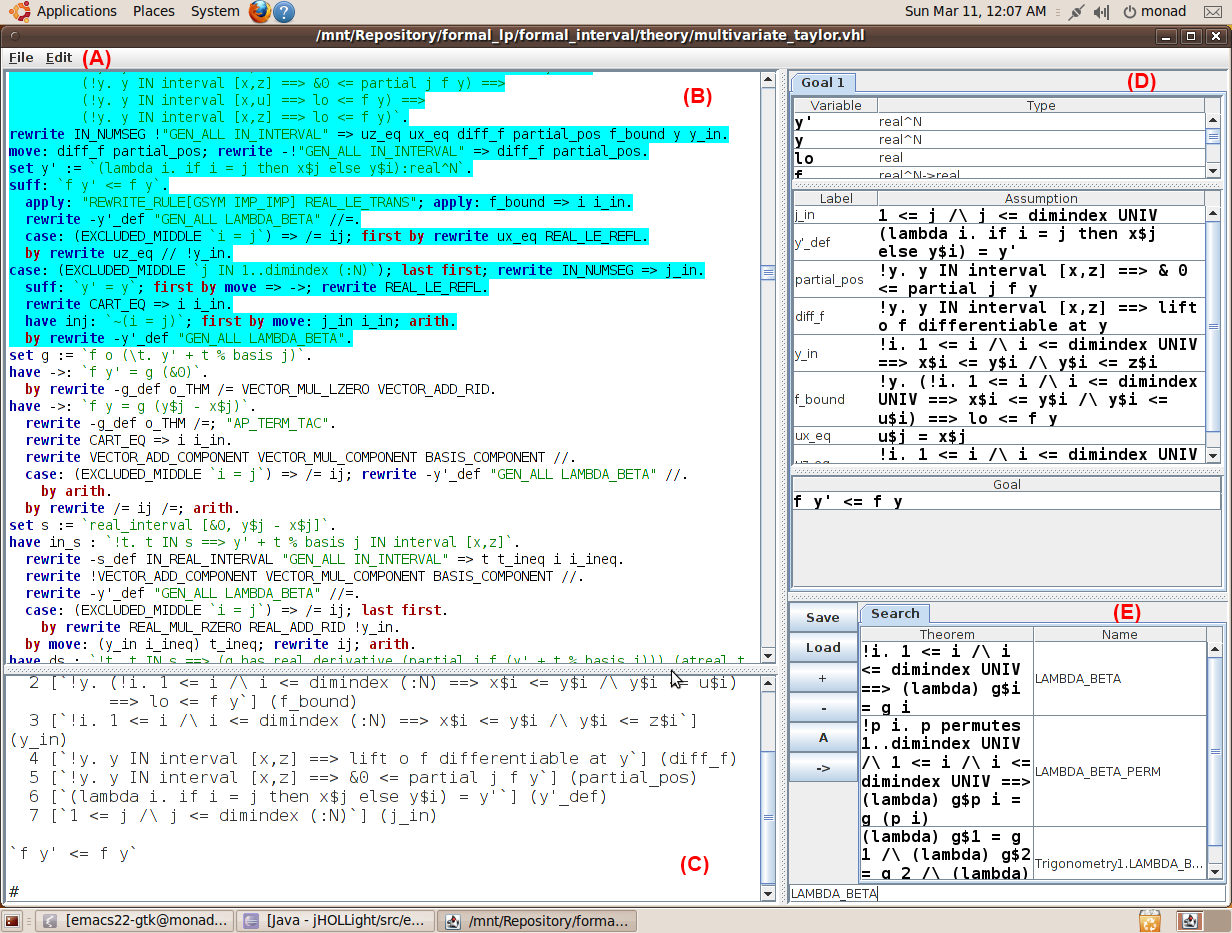
\includegraphics[width=\textwidth]{Screenshot.png}
\caption{SSReflect/HOL Light user interface.}
\end{figure}

The SSReflect/HOL Light user interface is shown at Figure 1. The main parts of the interface are: the main menu (A), the text editing area (B), the message area (C), the proof status area (D) which includes the list of context variable and the tabbed list of subgoals with assumptions, and the search area (E).


% Main Menu
\subsection{Main Menu}
The menu {\tt File} contains standard commands: create a new file, open an existing file, save changes, save changes in a new file (save as), exit the system. There is also a list of recently open files.

The menu {\tt Edit} contains the {\tt Highlight} checkbox. If this checkbox is selected, then the source code will be highlighted using SSRefelct/HOL Light rules. Note that the implementation of text highlighting is experimental in the current version of the system and works very slowly for relatively big source files.

% Text Editing
\subsection{Text Editing}
SSReflect/HOL Light script is a simple text file which contains special commands. Each command must be ended with a period symbol. When the period key \verb|.| is pressed during an editing process, then a period symbol will be printed and all unprocessed script text before this period symbol will be processed and the corresponding commands will be executed automatically. The output of the last command will be printed in the message area below the text editing area. If some error occurs during script processing or during command execution, then an error message will be printed in the message area and the process will stop at the command which caused the error. A processed script text will be marked with a special color. This part of the script cannot be modified unless some commands are undone. To undo the last command, press \verb|CTRL + Space|.
To undo several processed commands, move the cursor to a desired position inside a processed script text and press \verb|CRTL + Enter|. It will undo all commands up to the command at the cursor position (including this command) and the text corresponding to all these commands will become editable.

If the cursor is located right after a period symbol and the period key is pressed, then the script text will be processed but no additional period symbol will be printed. If you need to print a period symbol without text processing or need to print a period symbol after another period symbol (for example, when you enter a HOL Light term for a numerical segment in the form \verb|a..b|), then use the combination \verb|ALT + .| in order to print a period symbol. In general, it is not necessary to use this combination when entering HOL Light terms containing periods: a single period symbol will be always printed and an incomplete term expression will cause an error which can be ignored.

\issues
When a text is processed, then the system will be frozen until the process ends. You need to wait patiently, especially when loading some existing large HOL Light files in the system.

% Theorem Searching
\subsection{Theorem Searching}
The search area of the user interface can be used to find HOL Light theorems which contain special terms or have special names. All search request must be printed in the text field at the bottom of the search area. Each search request has the following form:
\begin{eqnarray*}
\xx{search\_request} &=& \xx{item}\ ...\ \xx{item}\\
\xx{item} &=& \xx{`term`} \mathrel{|} \xx{sequence\_of\_symbols}
\end{eqnarray*}
A search request is a list of search items separated by spaces. Each search item is either a back-quoted HOL Light term expression or a sequence of symbols which does not contain spaces (this sequence of symbols must be unquoted). The search function tries to find all theorems which contain all requested subterms and whose names contain all requested sequences of symbols.

Example: the search request \verb|`n + m` REAL| asks for all theorems which contain subterms of the form \verb|`n + m`| and whose names contain \verb|REAL|.

Search results can be organized using tabs. To add a new tab, press the \verb|+| button and enter tab's name. To delete an existing tab, select this tab and press the \verb|-| button. To make a tab active, select a tab and press the \verb|A| button. When a tab is active, then search result can be copied to that tab (it is also possible to copy results from one tab to another). To copy a search result, select it in the table of results and then press the \verb|->| button. This action will delete the selected result from the current table and copy it to the active tab table.

It is also possible to save the context of all tabs (excluding the first tab which contains most recent search results). Press the {\tt Save} button and select a file to save the context of tabs. Saved results can be loaded by pressing the {\tt Load} button.





% HOL Light scripts
\subsection{Producing HOL Light Scripts}
Translation of an SSReflect/HOL Light script into a HOL Light script is not very well developed yet. Now, there is only one way to obtain a HOL Light script from an SSReflect/HOL Light source file. Here is the instruction.

\begin{itemize}
\item[1] Open a source file, then process all commands in that file.
\item[2] Close the source file (open another source file, or quit the system).
\item[3] Go to the directory containing the source file. There should be a new file with the same name as the source file and with the {\tt .log} extension. This file contains all translated commands of the original source file.
\item[4] Rename the log file (for example, change its extension to {\tt .hl}).
\item[5] To load the renamed file in HOL Light, it is necessary to load the following files in HOL Light first: {\tt caml/ssreflect.hl} and {\tt caml/sections.hl}.
\end{itemize}



% General description
\section{SSReflect/HOL Light: General Description}

There are two main modes in the system: the declaration mode and the proof mode. In the declaration mode, it is possible to enter an arbitrary HOL Light (OCaml) command. In order to do so, a command need to be entered in quotes. If a HOL Light command itself contains quotes, then they need to be escaped and written as \verb|\"|. All commands in SSReflect/HOL Light must be ended with a period (\verb|.|) symbol. It includes raw HOL Light commands: a period must be placed after the closing quote. It is not necessary to end quoted HOL Light commands with \verb|;;|.

{\bf Examples:}
\begin{verbatim}
"needs \"lib.ml\"".
"let x_def = new_definition `x = 100`".
\end{verbatim}

Right now, there is no special mechanism for defining new objects in SSReflect/HOL Light. Standard HOL Light commands for making definitions must be used. Note that it is not possible to cancel or modified a HOL Light definition after it is made. You can go back in SSReflect/HOL Light script but all definitions should be not modified. If you need to modify a definition, then it will be necessary to restart SSReflect/HOL Light.

Standard OCaml comments \verb|(* *)| are available in SSReflect/HOL Light. This comments cannot be nested.

There are two things that can be done in the declaration mode. One thing is stating a lemma and starting its proof. Another thing is using section for organizing lemmas which share common variables and assumptions.

% Lemmas
\subsection{Lemmas}
A simple way to state a lemma and start its proof is the following:

\verb|Lemma lemma1 : `!x. x + 3 > 2`.|

This command starts a proof of a lemma with the given HOL Light statement. After a proof is complete, a new lemma will be called \verb|lemma1|. There should be no free variables in the statement of any lemma in SSReflect/HOL Light. The only exception is for variables which are declared as local section variables (more details later). All free variables of a lemma can be listed after lemma's name. In this way, the statement could be simpler in many cases:

\verb|Lemma lemma1 x : `x + 3 > 2`.|

Right now, it is not possible to specify types of variables which appear after lemma's name. So if you need some explicit type for a free variable, then all type information must be entered in the statement:

\verb|Lemma lemma2 x y : `x > y <=> ~(x = y) /\ x >= (y:real)`.|

When variables are listed after lemma's name, then they will be automatically generalized in the statement when the lemma is proved.

A proof has the following structure

\begin{verbatim}
Lemma lemma : `statement`.
Proof.
{tactics}
Qed.
\end{verbatim}

The keyword \verb|Proof| could be omitted. There is a small issue with this keyword: when \verb|Proof| is entered and \verb|.| is pressed, then an error message will be printed; this error should be ignored, and the \verb|Proof| keyword will be accepted after any valid tactic is entered after it. The \verb|Qed| keyword ends a proof. This keyword will work only if a lemma is completely proved. It is also possible to abort a proof by entering \verb|Abort| and pressing the period.


% Sections
\subsection{Sections}
A new section can be started with the command

\verb|Section name.|

Each section must be closed eventually. A section is closed by 

\verb|End name.| 

The {\tt name} should be exactly the same name used to open the section. Section may be nested.

Inside a section it is possible to declare local section variables and assumptions. All these variables and assumptions will be available to all lemmas which appear in that section and in all nested sections (it is true only for lemmas which appear after declarations of local variables and assumptions).

Local variables are declared by

\verb|Variable x : `:num`.|

\verb|Variables x y : `:real`.|

Types of all local variables must be explicitly given using a back-quoted HOL Light type expression. It is mandatory to put the colon right after the first back quote. The type expression \verb|`(:real)`| will give an error (this issue will be addressed in next versions of SSReflect/HOL Light). Keywords \verb|Variable| and \verb|Variables| are equivalent.

If a local variable \verb|x| is declared, then it will be possible to use this variable as a free variable in statements of lemmas. Also, its type is fixed, so it is possible to avoid explicit typing. All local variables will be generalized in statements of lemmas when the section where these local variables are declared is closed. 

{\bf Example:}
\begin{verbatim}
Section Vectors.

Variable x : `:real^N`.

Lemma lemma1 y : `x + y = y + x`.
Abort.

Lemma lemma2 : `&0 <= x dot x`.
Abort.

(* lemma2 = |- &0 <= x dot (x:real^N) *)

End Vectors.

(* lemma2 = |- !x:real^N. &0 <= x dot x` *)
\end{verbatim}

It is also possible to fix a type of a variable with the given name without creating a local variable. Use \verb|Implicit Type| instead of \verb|Variable| to do so. 

{\bf Example:}
\begin{verbatim}
Section Vectors.

Implicit Type x : `:real^N`.

(* The type of any variable with the name "x" is assumed to be `:real^N` *)
Lemma lemma1 x y : `x + y = y + x`.
Abort.

End Vectors.
\end{verbatim}

The keyword \verb|Hypothesis| is used to create a local section assumption.

\verb|Hypothesis h1 : `x > 0`.|

All variables in an assumptions must be bounded or they must be local variables declared before. So the example above will work only if \verb|x| is a local section variable with the correct type. All lemmas in a section proved after a given local hypothesis share this hypothesis. When the section is closed, then all hypotheses are discharged for all lemmas proved in that section. 

{\bf Example:}
\begin{verbatim}
Section Sect1.

Variable x : `:num`.
Hypothesis x_gt0 : `x > 0`.

Lemma lemma1 : `~(x = 0)`.
Proof. by move: x_gt0; arith. Qed.

(* lemma1 = x > 0 |- ~(x = 0) *)

Lemma lemma2 y : `y DIV x <= y`.
Proof. by rewrite (DIV_LE lemma1). Qed.

(* lemma2 = x > 0 | !y. y DIV x <= y *)

End Sect1.

(* lemma1 = |- !x. x > 0 ==> ~(x = 0) *)
(* lemma2 = |- !x. x > 0 ==> !y. y DIV x <= y *)
\end{verbatim}


% Proofs
\section{SSReflect/HOL Light: Proofs}
The proof mode is the main mode of SSReflect/HOL Light. As in the declaration mode, it is possible to use raw HOL Light commands and tactics in the proof mode. Again, all such commands must be quoted. The following HOL Light tactics might be helpful in SSReflect/HOL Light: \verb|"ANTS_TAC"|, \verb|"AP_TERM_TAC"|, \verb|"AP_THM_TAC"| (the last two tactics are used because the \verb|congr| tactic of SSReflect/Coq is not implemented in SSReflect/HOL Light now). Sometimes it is also necessary to modify a theorem before it can be used in SSReflect/HOL Light. For instance, it is important for rewriting that there are no free variables in a theorem statement. Most HOL Light theorems satisfy this condition, but in some cases it is wrong. In that situation, the following construction is helpful \verb|"GEN_ALL th"|. SSReflect/HOL Light does not infer types of quoted expressions. It just guesses the type based on a place where a quoted statement is used. This approach could lead to errors, but it is not a big issue. In general, quoted statements are rare inside SSReflect/HOL Light proofs. Eventually, I would like to completely eliminate them by providing appropriate tactics and, probably, special operators (for generalizing theorem variables, etc.).

There are two kinds of objects with which SSReflect/HOL Light tactics work: terms and theorems. Terms can be context variables or raw HOL Light terms. Theorems can be assumptions or HOL Light theorems.

% Terms
\subsection{Terms}
All free variables in a proof context (which include a goal term and all assumptions) are context variables. In general, when a HOL Light term is required, it must be entered as a back-quoted expression. For context variables, it is possible to use their names directly without any quotes. The system will recognize context variables and work with them as with usual terms. When a back-quoted term is used free variables are not allowed in such a term. The only exception are context variables and special wild cards. Also, if a variable in a term has the same name as some context variable, then it is assumed that these are the same variables and the type of the variable in the term is automatically derived from the context. For example, if the context has a variable \verb|x:real|, then the term \verb|`x + 2`| will be rejected since in this term expression the variable \verb|x| has type \verb|:num| which does not coincide with the type of the context variable \verb|x|. On the other hand, the term \verb|`x`| will be accepted and it will be interpreted as \verb|`x:real`|. There is no reason to introduce free variables about which nothing is known in the context. In fact, new variables can be introduced with a special tactic \verb|set| which creates abbreviations. This tactic introduces a new context variable and a fact about this variable: its definitional equality.

Back-quoted terms can have special wild cards. A wild card is just a variable name which starts with \verb|_|. Examples: \verb|_a|, \verb|_1|, or simply \verb|_|. Terms containing wild cards are allowed for several tactics (\verb|rewrite|, \verb|set|, \verb|:|). If a term contains a wild card, then it is treated as a pattern. This pattern is matched against the goal term. In this pattern matching all wild cards are free variables. If a match is found, then the matched term is used in a tactic. Note that wild cards with the same name must match the same goal subterm. For example, the pattern \verb|`_ = _`| matches only subterms of the form \verb|a = a|, and does not match anything like \verb|a = b|.


% Theorems
\subsection{Theorems}
A proof context contains assumptions. All assumptions in SSReflect/HOL Light must be labelled. In the current version of the system, it is possible to create several assumptions with the same label. This issue will be resolved in next versions of the system. Any assumption can be used as an argument of any tactic when a theorem is required. A labelled assumption behaves in the same way as a named HOL Light theorem.

There are two special ways to construct a new theorem from existing ones. The first construction is creation of conjunctions. If \verb$th1 = |- A$ and \verb$th2 = |- B$, then it is possible to write \verb|(th1, th2)|. This expression is a conjunction of two theorems: \verb$(th1, th2) = |- A /\ B$. This construction is not used very often. One example of its application is with the \verb|rewrite| tactic in the following way: \verb|rewrite (th1, th2)|. This tactic first tries to rewrite using the first conjunct (the first theorem) and if it fails, then the second conjunct is tried.

Theorems can be constructed by ``applying'' a theorem or a term to another theorem. The syntax is the following \verb|(th arg1 ... argn)|. The parentheses are required in most cases. The only exception is the tactic \verb|have| in the form \verb|have a := th arg1 ... argn|.

The ``application'' works as follows. First of all, \verb|(th arg1 arg2)| is the same as \verb|((th arg1) arg2)|. If a theorem has the form \verb$th = |- P ==> Q$ then \verb|arg1| must be a theorem of the form \verb$|- P'$ such that it is possible to match \verb|P'| and \verb|P|. The result of \verb|(th arg1)| is \verb$|- Q$. In this case, the ``application'' is equivalent to \verb|MATCH_MP th arg1|. If a theorem has the form \verb$th = |- !x. P x$, then the argument must be a term \verb|`y`|, and \verb|(th arg1)| will be \verb$|- P y$ (it is assumed that the type of \verb|`y`| is correct). In this case, the ``application'' is equivalent to \verb|ISPEC `y` th|. Note that if a theorem has the form \verb$th = |- !x. P x ==> Q x$ then it is possible to use ``application'' with a theorem which can match \verb|P x| directly. It is not required to specialize \verb|x| first. 

{\bf Example:}
\begin{verbatim}
th = |- !n. n < 2 ==> n = 0 \/ n = 1
arg = |- 0 < 2
(th arg) = |- 0 = 0 \/ 0 = 1
\end{verbatim}

% Chains of Tactics
\subsection{Chains of Tactics}
Tactics can be chained to form a single tactic. Chains of tactics are formed by adding a semicolon between two tactics \verb|tac1; tac2|. In this expression, if \verb|tac1| produces several subgoals, then \verb|tac2| is applied to all produced subgoals. It is possible to apply specific tactics to selected subgoals. It can be done with special tactical \verb|last| and \verb|first| (see the corresponding section) or it can be done with the following construction \verb$tac1; [tac2_1 | ... | tac2_k]$. Here $k$ is the number of subgoals produced by the first tactic. The $i$-th tactic in square brackets will be applied to the $i$-th subgoal.

\issues
In the construction \verb$[tac_1 | ... | tac_k]$ it is not possible to use empty tactics like \verb$[tac_1 | ]$. Use \verb|move| whenever a neutral tactic is required.

The construction \verb$by [tac_1 | ... | tac_k]$ is not supported.



% Introduction =>
\subsection{Introduction {\tt =>}}
The introduction tactical \verb|=>| is  used for introducing assumptions and for specializing variables.

\begin{eqnarray*}
&&\xx{tactic}\ \xx{=$>$}\ \xx{i-item}\ ...\ \xx{i-item}\\
\xx{i-item} &=& \xx{i-pattern} \mathrel{|} \xx{s-item} \mathrel{|} \xx{/view}\\
\xx{s-item} &=& \xx{/=}\ |\ \xx{//}\ |\ \xx{//=}\\
\xx{i-pattern} &=& \xx{ident}\ |\ \xx{\_}\ |\ 
				[\xx{occ-switch}]\xx{-$>$}\ |\ [\xx{occ-switch}]\xx{$<$-}\ |\ 
				\xx{[i-item $|$ ... $|$ i-item]}
\end{eqnarray*}

The tactic is executed before the introduction. All introductions are processed from left to right.

\verb|s-item| is a simplification operation. \verb|//| is translated into \verb|ASM_REWRITE_TAC[]|, \verb|/=| is translated into \verb|SIMP_TAC[]|, and \verb|//=| is translated into \verb|ASM_SIMP_TAC[]|. Note: \verb|//| is not exactly \verb|ASM_REWRITE_TAC[]|. If \verb|//| cannot solve a subgoal with \verb|ASM_REWRITE_TAC[]|, then it does not change anything in that subgoal.

\verb|/view| is a view which is applied to the top assumption of the goal after performing all previous introduction operations.

\verb|i-pattern| is used for introducing new facts as assumptions and for specialization of generalized variables. It will be explained by examples.

If the goal is \verb|P ==> Q|, then \verb|move => h| will introduce a new assumption \verb|h: P| and the goal becomes \verb|Q|. \verb|move => _| on the same goal will transform the goal into \verb|Q| without introducing a new assumption.

If the goal is \verb|!x. P x ==> Q| then \verb|move => y h| will specialize the variable \verb|x| and call it \verb|y| and then introduce a new assumption \verb|h: P y|. The goal becomes \verb|Q|.

\verb|->| and \verb|<-| can be used for rewriting during the introduction process. The tactic \verb|move: eq_th => ->| is equivalent to \verb|rewrite eq_th|, meanwhile \verb|move: eq_th => <-| is equivalent to \verb|rewrite -eq_th|. More precisely, if the goal is \verb|(a = b) ==> P a| then the tactic \verb|move => ->| transforms the goal into \verb|P b|. The occurrence switch works in the same way as in the \verb|rewrite| tactic.

\verb$[i1 | ... | in]$ is a branching \verb|i-pattern| if it is the first \verb|i-item| and the tactic is not \verb|move|. A branching \verb|i-pattern| applies introductions \verb|i1| to the first subgoal generated by the tactic, \verb|in| to the last subgoal generated by the tactic.

\verb$[i1 | ... | in]$ is a destructing \verb|i-pattern| if it is not the first \verb|i-item| or if the tactic is \verb|move|. A destructing \verb|i-pattern| executes a case splitting first (in the same way as the \verb|case| tactic) and then behaves like a branching \verb|i-pattern| for subgoals generated by the case splitting.

A tactic of the form \verb|rewrite th => [] []| is equivalent to \verb|rewrite th; case|. It is necessary to use two \verb|i-pattern|'s since the first \verb|i-pattern| is just an empty branching pattern.

If the goal is \verb|A /\ B ==> C| then \verb|move => [h1 h2]| introduces two assumptions \verb|h1: A| and \verb|h2: B| and transforms the goal into \verb|C|. The same effect can be obtained with either \verb|move => [] h1 h2|, \verb|move => [h1] h2|, or \verb|case => h1 h2|.

If the goal is \verb|(?x. P x \/ Q x) ==> R| then \verb$move => [t [hP | hQ]]$ produces two goals: the first goal is \verb|R| and it has an assumption \verb|hP: P t|, the second goal is \verb|R| and it has an assumption \verb|hQ: Q t|. This tactic can be written as \verb$case => t; case => [hP | hQ]$.


\issues
Suppose a goal is \verb|`(f x = 2) ==> f x < 3`|, then the following tactic will fail:
\verb|move => h1; rewrite h1|. The reason is that the system updates its knowledge about context variables and assumptions only after a chain of tactics is executed. In the example, \verb|rewrite h1| refers to the assumption \verb|h1| which is not known to the system when the chain of tactics is translated into a HOL Light tactic. During the translation process, the system assumes that \verb|h1| is a named HOL Light theorem and generates a tactic for rewriting with a theorem named \verb|h1|. Eventually, this issue will be resolved. Now, one must write \verb|move => h1. rewrite h1|.

It is possible to create different variables or assumptions with the same names: \verb|move => h h x x|. This will lead to a situation where one of assumptions or context variables could not be used directly.

% Discharge :
\subsection{Discharge {\tt :}}
The discharging tactical \verb|:| is used for discharging assumptions and for adding existing theorems as antecedents of a goal.

\begin{eqnarray*}
&&\xx{tactic} \xx{:} \xx{d-item}\ ...\ \xx{d-item}\\
\xx{d-item} &=& [\xx{occ-switch}](\xx{term}\ |\ \xx{th})
\end{eqnarray*}

The tactic before \verb|:| can be any tactic but the most common cases are \verb|move|, \verb|apply|, \verb|case|, \verb|elim|. The tactic is executed after discharging steps.

\verb|move: d1 d2 d3| is equivalent to \verb|move: d3; move: d2; move: d1|. The order of elements is reversed. It is done to make sure that the left-most element \verb|d1| becomes the left-most element in the goal after discharging. In this way, the tactic \verb|move: th1 th2 => h1 h2| creates two new assumptions \verb|h1: conclusion of th1| and \verb|h2: conclusion of th2|.

\verb|move: th| transforms a goal by adding the conclusion of the given theorem as an antecedent of the goal. It is equivalent to \verb|MP_TAC th|.

Assume that \verb|x| is a variable in the context, then \verb|move: x| transforms the goal by generalizing the variable \verb|x|. If the occurrence switch is used, then only specified occurrences of the variable are generalized. All other occurrences are renamed.

Note that \verb|x| will be generalized only in the goal, not in assumptions. If \verb|x| is used in some assumption and need to be generalized for that assumption as well, then this assumption must be discharged before generalization of \verb|x|.

\verb|move: `term`| finds all occurrences of the term (which can contain wildcards) in the goal. All these occurrences are replaced with a generated abbreviation, and then the abbreviation is generalized. The occurrence switch can be used to specify which subterms of the goal must be selected.

{\bf Examples:}

Goal: \verb|a + x = x + 3|

\verb|move: x| transforms the goal into \verb|!x. a + x = x + 3|.

\verb|move: {1}x a| transforms the goal into \verb|!x1 a. a + x1 = x + 3|, where \verb|x1| is an automatically generated name.

\verb|move: `x + 3`| transforms the goal into \verb|!x1. a + x = x1|.



% Views
\subsection{View {\tt /}}
Views in SSReflect/HOL Light provide only a very limited functionality of views in SSReflect/Coq. The primary reason is that there is no difference between Boolean values and propositions in HOL Light.

There are two main forms of views in SSReflect/HOL Light. The first form is \verb$tactic/theorem$. This is equivalent to the following tactic: 

\verb|move => top; move: (theorem top); move: top => _; tactic.|

Here \verb|top| is a fresh name. In other words, if a goal is \verb|P ==> Q| and \verb$th = |- P ==> R$, then \verb|move/th| transforms the goal into \verb|R ==> Q|.

The second form of views in SSReflect/HOL Light is \verb$tactic/(_ arg)$ where \verb|arg| is either a theorem or a term. This construction can be used if the top goal assumption has the form \verb|P ==> Q| or \verb|!x. P|. If a goal is \verb|(P ==> Q) ==> R| and \verb$th = |- P$, then \verb|move/(_ th)| transforms the goal into \verb|Q ==> R|. If a goal is \verb|(!x. P x) ==> Q|, then \verb|move/(_ y)| transforms the goal into \verb|P y ==> Q| (it is assumed that \verb|y| is a context variable). In the latter case, it is also possible to use raw HOL Light terms: \verb|move/(_ `y + 2`)|.

Views can also be used as introduction items after \verb|=>| (see the introduction tactical).



% by
\subsection{by}
\verb|by| is a tactical which has syntax \verb|by tactic|. Here \verb|tactic| can be a single tactic or a chain of tactics. \verb|by tactic| is equivalent to \verb|tactic; done|. This tactical is used to ensure that a current subgoal is completely proved. It is a good practice to end any subgoal proof with \verb|by| or any other tactic which fails when a goal is not proved (\verb|exact|, \verb|arith|, \verb|done|).


% try
\subsection{try}
\verb|try| tries to apply a tactic and does nothing if the tactic fails.

Syntax: \verb|try tactic|

\verb|tactic| must be a single tactic, not a chain of tactics.

{\bf Example:}

\verb|try arith| solves all subgoals which can be solved with \verb|arith|.


% last, first
\subsection{last, first}
\verb|last| (\verb|first|) applies a given tactic to the last (first) subgoal in a goal stack.

Syntax:
\verb|last tac|, \verb|first tac|

Note that \verb|tac| must be a single tactic, not a chain of tactics. For example, the expression 

\verb|case; last rewrite th1; rewrite th2| 

works as follows: \verb|case| is applied, \verb|rewrite th1| is applied to the last subgoal and then \verb|rewrite th2| is applied to all subgoals. On the other hand, 

\verb|case; last by rewrite th1; rewrite th2| 

works differently: \verb|rewrite th1; rewrite th2| is applied to the last subgoal only (since the chain of these two tactics form a single argument of the \verb|by| tactical).

\issues
It is not possible to use parentheses in order to parse a chain of tactics as a single tactic for \verb|last| or \verb|first|.


% last first
\subsection{last first, first last}
\verb|last first| (\verb|first last|) rotates the goal stack.

Syntax: $\xx{last} [\xx{n}] \xx{first}$, $\xx{first} [\xx{n}] \xx{last}$.

By default, the number $n$ is 1.

If a goal stack has subgoals $g_0, g_1, \ldots g_{k - 1}$, then \verb|first [n] last| transforms the goal stack to $g_{0 + n}, g_{1 + n}, \ldots, g_{(k - 1) + n}$. Here, $i + n$ is computed modulo $k$.

If a goal stack has subgoals $g_0, g_1, \ldots, g_{k - 1}$, then \verb|last [n] first| transforms the goal stack to $g_{0 - n}, g_{1 - n}, \ldots, g_{(k - 1) - n}$. Here, $i - n$ is computed modulo $k$.

If there are only two goals in the stack, then \verb|last first| and \verb|first last| are equivalent.


% do
\subsection{do}
\verb|do| repeats a given tactic.

\begin{eqnarray*}
&&\xx{do}\ [\xx{mult}]\ \xx{[tactic $|$ ... $|$ tactic]}\\
\xx{mult} &=& [\xx{n}](\xx{!}\ |\ \xx{?})
\end{eqnarray*}

When a list of parallel tactics is used, then \verb$do [tac1 | tac2 ... | tac_n]$ executes the first tactic which is successful.

By default, the tactic is executed only one time. The multiplier \verb|mult| specifies how many times the tactic should be repeated. The key \verb|!| specifies that the tactic must be performed at least one time and then repeated as many times as possible. An explicit number before this key specifies how many times the tactic should be repeated exactly. The key \verb|?| specifies that the tactic must be repeated as many times as possible (even 0 times). An explicit number before this key specifies the maximum number of times the tactic should be repeated. Note: if no explicit number is given then the tactic is repeated at most 10 times for both keys (this limitation is introduced to prevent infinite loops for some tactics).

% left
\subsection{left, right}
\verb|left| transforms a goal \verb|A \/ B| into \verb|A|; \verb|right| transforms a goal \verb|A \/ B| into \verb|B|.

Implementation notes: \verb|left| and \verb|right| correspond to HOL Light tactics \verb|DISJ1_TAC| and \verb|DISJ2_TAC| respectively.

% split
\subsection{split}
If \verb|split| is applied to a goal \verb|A /\ B|, then two new subgoals are created: \verb|A| and \verb|B|. If \verb|split| is applied to a goal \verb|A <=> B|, then two new subgoals are created: \verb|A ==> B| and \verb|B ==> A|.

Implementation notes: \verb|split| is translated into \verb|split_tac| which is defined as follows

\verb|let split_tac = FIRST [CONJ_TAC; EQ_TAC];;|


% exists
\subsection{exists}
\verb|exists| provides witnesses for existential quantifiers.

$$\xx{exists}\ \xx{term}\ ...\ \xx{term}$$

{\bf Examples:}

Goal: \verb|?a b. a > SUC b|

\verb|exists `3` `1`| transforms the goal into \verb|3 > SUC 1|.

\verb|exists x `1 + y`| transforms the goal into \verb|x > SUC (1 + y)| (variables \verb|x| and \verb|y| must appears in the context and have type \verb|:num|).

\verb|exists x| transforms the goal into \verb|?b. x > SUC b|. This will work only if \verb|x| appears in the context and its type is \verb|:num|.


% done
\subsection{done}
\verb|done| proves trivial goals and fails if it cannot prove a goal.

Implementation notes: \verb|done| is translated into \verb|done_tac| which is defined as follows

\verb|let done_tac = ASM_REWRITE_TAC[] THEN FAIL_TAC "done";;|


% arith
\subsection{arith}
\verb|arith| is a tactic for proving basic algebraic statements for natural, real, and integer numbers. This tactics fails if it cannot solve a goal.

{\bf Example:}

The goal \verb|a + a = &2 * a| is solved by \verb|arith.|

Implementation notes: \verb|arith| is translated into \verb|arith_tac| which is defined as follows

\verb|let arith_tac = FIRST [ARITH_TAC; REAL_ARITH_TAC; INT_ARITH_TAC];;|


% move
\subsection{move}
\verb|move| does virtually nothing. It is used in conjunction with tactical \verb|=>| and \verb|:| for introducing and discharging assumptions.

Implementation notes: \verb|move| is translated into \verb|BETA_TAC|.


% set
\subsection{set}
\verb|set| introduces an abbreviation.

$$\xx{set}\ \xx{name}\ \xx{:=}\ \xx{`term`}$$

The left hand side should be a fresh name, the right hand side is a back-quoted HOL Light term which can contain wild cards \verb|_|. Types of all free variables of the term are instantiated based on the types of context variables.

Wild cards in the term are used for matching the term against the current goal. If a match is found for a subterm in the goal, then the matched term is used in the definition.

If the tactic \verb|set| is successful, then a new equation will be added to the list of assumptions. This equation will have the label \verb|name_def| and it will be of the form \verb|term = name|.

{\bf Examples:}

Goal: \verb|SUC (1 + f x y + 2) = 3|

\verb|set g := `f x y`| introduces a new assumption \verb|g_def: f x y = g| and changes the goal to \verb|SUC (1 + g + 2) = 3|.

\verb|set g := `_ + 2`| introduces a new assumption \verb|g_def: f x y + 2 = g| and changes the goal to \verb|SUC (1 + g) = 3|


% have
\subsection{have}
\verb|have| introduces a new subgoal.

$$\xx{have}\ [\xx{label}]\xx{:}\ \xx{`term`}$$

This tactic creates a new subgoal defined by the term and adds the same assumption to the original goal with the given label. The label could be omitted. In that case, the statement of the subgoal is added as an antecedent to the original goal.

There is another form of this tactic which can be used for adding an existing theorem into a list of assumption: \verb$have label := thm$

{\bf Examples:}

Goal: \verb|P (1 + x) = r|

\verb|have: `1 + x = 3`| creates a new subgoal \verb|1 + x = 3| and changes the original goal to \verb|1 + x = 3 ==> P (1 + x) = r|.

\verb|have h1 := ETA_AX f| creates a new assumption with the label \verb|h1| which corresponds to the given theorem. Note that it is not required to put parentheses around \verb|ETA_AX f|.


Implementation notes: \verb|have| syntax is more complex. It is possible to write \verb|have [] [a b]: `A /\ B`|. This corresponds to the destructive pattern matching of the introduction tactical \verb|=>|. I plan to make the syntax and the behaviour of \verb|have| closer to its counterpart in Coq/SSReflect, so it is recommended to use only the basic forms of this tactic.


% suff
\subsection{suff}
\verb|suff| is a variation of \verb|have|.

\verb|suff| switches two goals generated by \verb|have|, i.e., \verb|suff| is equivalent to an application of \verb|first last| after \verb|have|.


% wlog
\subsection{wlog}
\verb|wlog| is a variation of \verb|have|.

$$\xx{wlog}\xx{:}\ \xx{id\_list}/\xx{`term`}$$

\verb|id_list| is a list of identifiers (variable names) which can be empty.

\verb|wlog: / `Q`| transforms a goal \verb|`P`| into two subgoals \verb|`(Q ==> P) ==> P`| and \verb|`Q`|.

\verb|wlog: n1 n2 / `Q`| transforms a goal \verb|`P`| into two subgoals \verb|`(!n1 n2. Q ==> P) ==> P`| and \verb|`Q`|.



% case
\subsection{case}
\verb|case| performs a case analysis on the first antecedent or on the top universally quantified variable of a goal.

The behaviour of \verb|case| depends on the form of a goal.

\verb|case| transforms a goal \verb|A /\ B ==> C| into \verb|A ==> B ==> C|.

\verb|case| transforms a goal \verb|A \/ B ==> C| into \verb|A ==> C| and \verb|B ==> C|.

\verb|case| transforms a goal \verb|(?x. P x) ==> Q| into \verb|!x. (P x ==> Q)|.

\verb|case| transforms a goal \verb|!n:num. P n| into two subgoals \verb|P 0| and \verb|!m. P (SUC m)|.

\verb|case| transforms a goal \verb|!a:(A)list. P a| into two subgoals \verb|P []| and \verb|!h t. P (CONS h t)|.

\verb|case| transforms a goal \verb|!a:A#B. P a| into \verb|!(x:A) (y:B). P (x, y)|.

It is common to combine \verb|case| with \verb|=>| and \verb|:| tacticals.

{\bf Examples:}

Goal: \verb|(?x. P x) ==> Q|

\verb|case => y hP| changes the goal into \verb|Q| and creates an assumption \verb|hP: P y|.

Goal: \verb|P (x + 2)|

\verb$case: (EXCLUDED_MIDDLE `x + 2 = 3`) => [-> |]$ transforms the goal into two subgoals
\verb|P 3| and \verb|~(x + 2 = 3) ==> P (x + 2)|.

Implementation notes: \verb|case| is translated into \verb|case_tac|. SSReflect/HOL Light implementation of \verb|case| is not as powerful as the original implementation in Coq/SSReflect. \verb|case_tac| can handle only a predefined number of situations meanwhile the original \verb|case| tactic in Coq/SSReflect works for any inductive type. The current implementation of \verb|case_tac| covers most common situations when this tactic can be applied. It will be pretty easy to extend the current implementation if it becomes necessary.


% elim
\subsection{elim}
\verb|elim| performs an inductive elimination on the top universally quantified variable of a goal.

This tactic works only for variables of \verb|:num| and \verb|:(A)list| types.

\verb|elim| transforms a goal \verb|!n:num. P n| into two subgoals: 

\verb|P 0| and \verb|!n. P n ==> P (SUC n)|.

\verb|elim| transforms a goal \verb|!a:(A)list. P a| into two subgoals: 

\verb|P []| and \verb|!a0 a1. P a1 ==> P (CONS a0 a1)|.


% apply
\subsection{apply}
\verb|apply| corresponds to \verb|MATCH_MP_TAC|.

\verb|apply| transforms a goal \verb|(P ==> Q') ==> Q| into \verb|P| if \verb|Q'| can be matched to \verb|Q|.

If a goal has the form \verb|(P ==> Q ==> R) ==> X|, then the tactic first tries to match \verb|X| with \verb|Q ==> R|. If this fails, then the antecedent is transformed into \verb|P /\ Q ==> R| and the process repeats.

There is another form of the tactic: \verb|apply th|. In this case, it is completely equivalent to \verb|MATCH_MP_TAC th|. It was necessary to introduce this form since HOL Light cannot handle assumptions with polymorphic types. Here is an example:

Goal: \verb|!a:(num)list. P a|. Then the tactic \verb|apply list_INDUCT| works and transforms the goal into \verb|P [] /\ (!a0 a1. P a1 ==> P (CONS a0 a1))|. The tactic \verb|apply: list_INDUCT| fails on the goal. The reason is that the tactical \verb|:| adds a new theorem as an antecedent of the goal, and then \verb|apply| tries to use this antecedent to match the original conclusion. Matching is successful, but the matched theorem now has the form \verb$P[:num/:A] |- P[:num/:A]$ meanwhile the list of assumptions contains the original polymorphic version of the theorem and the tactic fails.


% exact
\subsection{exact}
This tactic is equivalent (with some limitation) to the construction 

\verb$do [done | by move => top; apply top]$ 

where \verb|top| is a fresh name.

\verb|exact| is often used to finish a subgoal proof.

Implementation notes: \verb|exact| is translated into \verb|exact_tac| which is defined as

\verb|FIRST [done_tac; DISCH_THEN (fun th -> apply_tac th) THEN done_tac];;|


% rewrite
\subsection{rewrite}
\verb|rewrite| uses an equational theorem to change a goal.

\begin{eqnarray*}
&&\xx{rewrite}\ \xx{r-step}\ ...\ \xx{r-step}\\
\xx{r-step} &=& [\xx{r-prefix}]\xx{r-item}\\
\xx{r-prefix} &=& [\xx{-}]\ [\xx{mult}]\ [\xx{occ-switch}]\ [\xx{[`term`]}]\\
\xx{occ-switch} &=& \xx{\{$n_1$ ... $n_k$\}}\\
\xx{r-item} &=& \xx{theorem}\ |\ \xx{s-item}\\
\xx{s-item} &=& \xx{/=}\ |\ \xx{//}\ |\ \xx{//=}
\end{eqnarray*}

\verb|rewrite r1 r2| is equivalent to \verb|rewrite r1; rewrite r2|.

The most basic form of the tactic is \verb|rewrite th| where \verb|th| is an equational HOL Light theorem. The tactic tries to find a subterm in the goal which matches the left hand side of the provided theorem. If a matching subterm is found, then the theorem is instantiated such that its left hand side becomes equal to the matching subterm and all instances of the left hand side of the theorem in the goal are replaced with theorem's right hand side. Free variables of the theorem are not instantiated during rewriting.

In fact, \verb|th| could be any theorem. If it is a conjunction of several results, then the tactic tries all conjuncts and it stops after first successful rewriting. If the given theorem is not an equational theorem of the form \verb$|- P$ then it is transformed into the theorem \verb$|- P <=> T$ before rewriting. A theorem of the form \verb$|- ~P$ is transformed into \verb$P <=> F$.

\verb|rewrite| works for theorems with assumptions. If \verb$th = |- P ==> (f = g)$, then \verb|rewrite th| changes all occurrences of \verb|f| to \verb|g| in a goal and introduces a new subgoal \verb|P|.

The \verb|-| switch changes the direction of rewriting. It is equivalent to an application of \verb|GSYM| to a theorem before rewriting.

The occurrence list \verb|occ-switch| specifies which occurrences of a matched term should be rewritten. This list must contain natural numbers separated by spaces.

The term \verb|[`term`]| in square brackets must be a back-quoted HOL Light term which may contain wild cards. Types of all free variables in this term are instantiated to the types of the corresponding context variables. If this term is provided, then the tactic finds a matching term in a goal and then searches for rewrites only inside this subterm.

By default, the tactic is executed only one time for the given theorem. It is possible to repeat the rewriting process several times. The exact number of repetitions is controlled by the multiplier \verb|mult| which has the same syntax and behaviour as for the \verb|do| tactic.

It is important to remember that free variables of a given theorem are not instantiated in matching and rewriting processes. If a theorem contains free variables in the left hand side, then they must correspond to the same variables in a goal. Some HOL Light theorems are not generalized, so it is required to use the following construction to work with such theorems

\verb|rewrite "GEN_ALL REAL_MUL_ASSOC"|

The fact that free variables of a theorem must coincide with free variables of a goal helps to make rewriting of manually selected subterms. Consider an example:

Goal: \verb|a = &3 * a|

\verb|rewrite -(REAL_MUL_LID `&3`)| transforms the goal into \verb|a = (&1 * &3) * c|, meanwhile
\verb|rewrite -REAL_MUL_LID| transforms the goal into \verb|&1 * a = &3 * &1 * a| since the pattern matching follows the left hand side first rule and it finds the first appropriate subterm \verb|`a`| and replaces all occurrences of this subterm. Another way to get the first result is to use a pattern: \verb|rewrite -[`&3`]REAL_MUL_LID| or \verb|rewrite -[`& _`]REAL_MUL_LID|.

\verb|rewrite -{2}REAL_MUL_LID| transforms the goal into \verb|a = &3 * &1 * a| since only the second occurrence of the matched term \verb|`a`| is asked to be replaced. \verb|rewrite -{2}(REAL_MUL_LID `&3`)| will not work since there is only one occurrence of the term \verb|`&3`| in the goal.


\issues
Conditional rewriting could fail when a subterm is rewritten inside an abstraction. This happens because the current implementation of rewriting does not appropriately rename bound variables.

\verb|rewrite ETA_AX| does not simplify subterms of the form \verb|`\x. f a x`|. To simplify such a subterm, use \verb|rewr ETA_AX|.


% rewr
\subsection{rewr}
\verb|rewr th| is directly translated into \verb|ONCE_REWRITE_TAC[th]|.

This tactic has a limited number of applications. Sometimes \verb|rewrite| fails or does not work in simple cases (e.g., \verb|rewrite ETA_AX|), then \verb|rewr| can be used. \verb|rewr| allows chains of rewrites and it supports multipliers \verb|[n]!| and \verb|[n]?|.



\end{document}



